\section{$\Delta$QSD implementation}
    A probe's $\Delta$Q can be represented internally by a PDF and displayed as an ECDF. Here is how both can be calculated given $n$ outcome instances.
    
    \subsubsection{PDF}
  We approximate the PDF of the observed $\Delta$Q via a histogram. We partition the values into $N$ bins of equal width, Given $\lbrack x_i, x_{i+1} \rbrack$ the interval of a bin $i$, where $x_i = i\Delta t$, and $\hat{p}(x_i)$ the value of the PDF at bin $i$, for $n$ bins:
        \begin{equation}
            \begin{cases}
                \hat{p}(i) = \dfrac{s_i}{n}, \text{if } i \le n \\
                \hat{p}(i) = 0, \text{if } i > n \\
            \end{cases}
            \label{eq:pdf}
        \end{equation}
    Where $s_i$ the number of successful outcome instances whose elapsed time is contained in the bin $i$, $n$ the total number of instances. \cite{stat}

    \subsubsection{ECDF}
        The value $\hat{f}(x_i)$ of the ECDF at bin $i$ with $n$ bins can be calculated as:
        \begin{equation}
            \begin{cases}
                \hat{f}(i) = \sum_{j=1}^{i} \hat{p}(j), & \text{if } i \le n \\  
                \hat{f}(i) = \hat{f}(x_n), & \text{if } i > n 
            \end{cases}
            \label{eq:cdf}
        \end{equation}

    \subsection{dMax}
        We introduced $dMax$ in the previous section, we provide here the full equation that allows $dMax$ to be calculated:
        \begin{equation}
            dMax = \Delta_{t base} * 2^n * N  
            \label{eq:dMaxU}
        \end{equation}
        Where:
        \begin{itemize}
            \item $\Delta_{t base}$ represents the base width of a bin, equal to 1ms.
            \item $N$ the number of bins.
        \end{itemize}


      \subsection{Operations}
    In a previous section we talked about the possible operations that can be performed on and between $\Delta$Qs, the time complexity of FTF, ATF and PC is trivially $\mathcal{O}(N)$ where N is the number of bins.
    
    As to convolution, the naïve way of calculating convolution has a time complexity of $\mathcal{O}(N^2)$, this quickly becomes a problem as soon as the user wants to have a more fine-grained understanding of a component. Below we present two ways to perform convolution.

        \subsubsection{Convolution} \label{convol}
        
        \paragraph{Naïve convolution}
        Given two $\Delta$Q binned PDFs $f$ and $g$, the result of the convolution $f \circledast g$ is given by \cite{conv}: 
        \begin{equation}
            (f \circledast g)\lbrack n \rbrack = \sum_{m = 0}^{N} = f\lbrack m \rbrack g \lbrack n - m \rbrack  
            \label{eq:discconv}
        \end{equation}
 
    \paragraph{Fast Fourier Transform Convolution}
        FFTW (Fastest Fourier Transform in the West) is a C subroutine library \cite{fftw3} for computing the discrete Fourier Transform in one or more dimensions, of arbitrary input size, and of both real and complex data. We use FFTW in our program to compute the convolution of $\Delta$Qs. We adapt our script from an already existing one found on GitHub. \cite{fft}
    
    Whilst the previous algorithm is far too slow to handle a high number of bins, convolution leveraging Fast Fourier Transform (FFT) allows us to reduce the amount of calculations to $\mathcal{O}(n \text{log} n)$. This is why the naïve convolution algorithm is not used. We will analyse the time gains in a later chapter.
    
    FFT and naïve convolution produce the same results in our program barring $\varepsilon$ differences (around $10^{-18}$) in bins whose result should be 0.
    
    FFTs algorithms are plenty, the choice of the one to use is left up to the subroutine via the parameter \texttt{FFTW\_ESTIMATE} \cite{fft-h}.

    \subsubsection{Arithmetical operations}
        We can apply a set of arithmetical operations between $\Delta$Qs ECDFs, and on a $\Delta$Q.
    \paragraph{Scaling (multiplication)} A $\Delta$Q can be scaled w.r.t. a constant $0 \le j \le 1$. It is equal to binwise multiplication on ECDF bins.
    \begin{equation}
        \hat{f_r}(i) = \hat{f}(i) \cdot j
        \label{eq:mul_ecdf}
    \end{equation}

    \paragraph{Operations between $\Delta$Qs} 
        Addition, subtraction and multiplication can be done between two $\Delta$Q of equal bin width (but not forcibly of equal length) by calculating the operation between the two ECDFs of the $\Delta$Qs:
        \begin{equation}
            \Delta \text{Q}_{AB}(i) = \hat{f_A}(i) [\cdot, +, -] \hat{f_B}(i)
            \label{eq:op_dq}
        \end{equation}


    \subsection{Confidence bounds}
        Here is how we calculate the mean and lower/upper confidence for the $\Delta$Qs ECDF at bin $i \quad \forall i < N$. \cite{stat}

        For $x_{ij}$ the value of an ECDF $j$ at bin $i$, the mean of all ECDFs for the bin over a window is:
            \begin{equation}
                \mu_i = \dfrac{1}{n_i} \sum_{j=1}^{n_i} x_{ij}
                \label{eq:mean_ecdf}
            \end{equation}
        Its variance:
            \begin{equation}
                \sigma^2_i = \dfrac{1}{n_i} \sum_{j=1}^{n_i} x^2_{ij} - \mu^2_i
                \label{eq:var_ecdf}
            \end{equation}
        The confidence intervals $CI_i$ for a bin $i$ can then be calculated as:
        \begin{equation}
            CI_i = \mu_i \cdot \dfrac{\sigma_i}{\sqrt{n_i}}      
            \label{eq:ci_i}
        \end{equation}

        \subsection{Rebinning}
            Rebinning refers to the aggregation of multiple bins of a bin width $i$ to another bin width $j$. 
            Operations between $\Delta$Qs can be done on $\Delta$Qs that have the same bin width, this is why it is fundamental that all probes have a common $\Delta_{tbase}$. This allows for fast rebinning to a common bin width. \\
            Given two $\Delta$Qs $\Delta$Q$_i$, $\Delta$Q$_j$:
            \begin{center}
                $\Delta_{Tij}$ = max \{$\Delta_{Ti}, \Delta_{Tj} \}$
            \end{center}
            and the PDF of the rebinned $\Delta$Q at bin $b$, from the original PDF of $n$ bins, where $k$ = $\frac{\Delta{_Ti}}{\Delta_{Tj}}$:
            \begin{equation}
                p'_b = \sum_{n=b \cdot k}^{b+ 1 \cdot k - 1} p_n, \quad b=0,1,\dots \lceil \frac{N}{k} \rceil  
            \end{equation}
            We perform rebinning to a higher bin width for a simple reason, while this leads to loss of information for the $\Delta$Q with the lowest bin width, rebinning to a lower bin width would imply inventing new values for the $\Delta$Q with the highest bin width.
        \begin{figure}[H]
            \centering
            \begin{subfigure}{.5\textwidth}
                \centering
                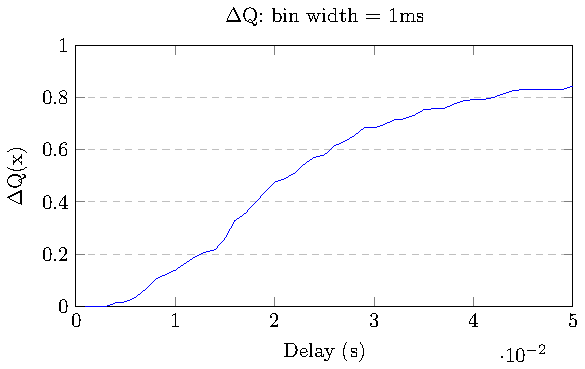
\includegraphics[width =0.98\textwidth]{tikz/cdf.pdf}
                \label{fig:nrb}
                \subcaption{Sample $\Delta$Q with 1ms bins}%
            \end{subfigure}%
            \begin{subfigure}{.5\textwidth}%
                \centering%
                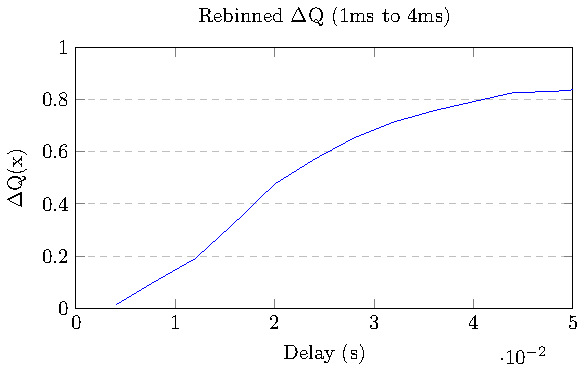
\includegraphics[width =0.98\textwidth]{tikz/rebinned_cdf.pdf}%
                \label{fig:sub2}%
                \subcaption{$\Delta$Q on the left after rebinning to 4ms bins}%
            \end{subfigure}%
            \label{fig:w1w2hb}%
            \end{figure}%


